\section{Multi-objective Weight Optimization}
\label{sec:multiobjective}

With an accurate CPU model, the weights must now be tuned to match measured
power consumption on real hardware. We formulate this as a multi-objective
optimization problem.

We start by creating a set of training workloads, essentially computer programs
designed to hold certain characteristics compiled to a native
ARMv7\footnote{ARMv7 is the instruction set supported by ARM Cortex-A9.} binary.
The design and selection of these will be elaborated in the next section. We
execute the binaries in the gem5 simulator with the CPU model from last
section to obtain a file containing \texttt{(time, event)} tuples from the
(modeled) execution, just like in \autoref{lst:trace}. The next challenge is to
assign each of these events a cost.

We attack this problem by running a multi-objective optimization algorithm. We
pick a subset of event types that is believed to impact energy consumption, as
we described in \autoref{subsec:powerevents}. Choosing too many events could
give us overfitting issues, but taking too few out could lead to lack of detail
in our model. We experimented with dozens of optimization algorithms and ended
up combining a $1 + \lambda$ evolutionary strategy with simulated annealing. The
evolutionary part would make sure that our algorithm was explorative enough
(i.e. it covered large parts of the solution space), while the simulated
annealing part made the algorithm more aggressive to start with. Using DEAP
\cite{DEAP_JMLR2012}, a Python framework for evolutionary algorithms, we were
able to prototype our ideas rapidly. \autoref{lst:ga-algorithm} describes the
final algorithm.

\begin{algorithm}
\caption{Algorithm used to evolve a set of event weights.}
\label{lst:ga-algorithm}
\begin{lstlisting}[language=python,style=algo]
individuals = createIndividuals()
generations = 6000

best = None
for 1 to generations:
    for ind in individuals:
        evaluate(ind)
        if ind betterthan best:
            best = ind
    individuals = mutate(ind)

print best
\end{lstlisting}
\end{algorithm}

\begin{figure}
    \centering
    \def\svgwidth{\columnwidth}
    \includegraphics[width=0.8\textwidth]{figs/ga_genome.pdf}
    \caption{Sample individuals.}
    \label{fig:ga-genome}
\end{figure}

Each individual is a set of CPU events, each mapped to an energy cost.
\autoref{fig:ga-genome} illustrates what individuals in the population look
like. The top row enumerates all event types; e.g. the cost of an integer
multiply event for individual 2 is 1400. The unit here is not really important,
but roughly corresponds to $Ampere * cycles$, with static drain deducted. The
evolutionary algorithm starts by generating 10 individuals by using the
algorithm shown in \autoref{lst:ga-create-algorithm}. Basically, it assigns most
weights a random value in range $\{0, \ldots, 999\}$, while guiding some weights
to a known value. E.g. the static energy contribution is known to lie around 96
mA by physical measurements, so its weight is believed to be close to that
number. Please note that there is not necessarily a direct mapping between the
GA weights and measured milliamperes; it is up to the evolutionary algorithm to
figure out what causes a best fit.

\begin{algorithm}
\caption{Algorithm used to generate individuals.}
\label{lst:ga-create-algorithm}
\begin{lstlisting}[language=python,style=algo]
#Properties kept by each individual
individualProperties = {
    'IntAlu', 'IntMult', 'IntAlu', 'IntMult', 'MemRead', 'MemWrite',
    'SimdFloatMisc', 'L1IR', 'L1IW', 'L1DR', 'L1DW', 'L2R', 'L2W',
    'PhysR', 'PhysW', 'Static', 'Idle'}

#Generate random individual
def createIndividual():
    ind = EmptySet
    for prop in individualProperties:
        ind[prop] = random()*1000
    ind['Static'] = 96*(random()+0.5)
    ind['Idle'] = 50*(random()+0.5)
    return ind

#Generate 10 random individuals
def createIndividuals():
    individuals = EmptyList
    for 1 to 10:
        individuals.add(createIndividual())
    return individuals
\end{lstlisting}
\end{algorithm}

To calculate the fitness of an individual, we run PET with the genome weights on
a set of workloads and compare the energy profiles with measurements on
hardware. The two sets are then compared using \autoref{lst:ga-eval-algorithm},
resulting in the individual fitness (lower is better).

\begin{algorithm}
\caption{Algorithm used to evaluate an individual.}
\label{lst:ga-eval-algorithm}
\begin{lstlisting}[language=python,style=algo]
#Evaluate individual
tests = {'trend', 'submul', 'sha2', 'pi'}

#Find RMS distance between two datasets
def distance(graph1, graph2):
    diff = 0
    for points in graph1, graph2:
        diff += (points[1] - points[2])^2
    return sqrt(diff / minsizeof(graph1, graph2));

#Find RMS distance between PET estimate and measured power consumption
def runTest(ind, test):
    data = runPET(getWeights(ind), test)
    measure = getMeasureData(test)
    return rmsDiff(data, measure)

#Find all distances and return result as RMS
def evaluate(ind):
    fitness = 0
    for test in tests:
        testFit =  runTest(ind, test)k
        fitness = fitness + testFit^2
    return sqrt(fitness)
\end{lstlisting}
\end{algorithm}


%TODO: Figure out if we need this
%\begin{algorithm}
%\caption{Algorithm used to mutate individuals}
%\label{lst:ga-mutate-algorithm}
%\begin{lstlisting}[language=python,style=algo]
%#Mutate individual, each property with a given probability
%def mutate(ind, probability):
%    mutateDegree = ind.fitness^1.4 + 100
%    for prop in individualProperties:
%        if random() < probability:
%            ind[prop] = ind[prop] + ( (random()-0.5) * mutateDegree)
%    return ind
%\end{lstlisting}
%\end{algorithm}


We emphasize that the use of an evolutionary algorithm is an arbitrary choice;
technically, we could have picked any algorithm to do this for us. When the
weights have evolved to match our hardware measurements, we no longer care how
these weights were obtained.
